% this is a comment!!!
% these don't appear in your final rendered document


\documentclass{article} % Starts an article
\usepackage{amsmath} % Imports amsmath


% enables text wrapping
\usepackage{url}

\usepackage{graphicx} % takes care of graphic including machinery

\usepackage{subfig}

\usepackage[margin=1in,letterpaper]{geometry} % decreases margins

\title{\LaTeX Introduction} % Title
% \LaTeX prints LaTeX all fancy like
\author{Jeffery Russell}

\begin{document} % Begins a document
  \maketitle % places document at start of file
  \LaTeX{} is a document preparation system for
  the \TeX{} typesetting program.

\section{Math}

	In \LaTeX, there are tons of options for writing math.
	Over time you will memorize a lot of them, however, TexMaker has a side panel with all the math symbols. Math can be done in-line with single dollar signs like this: $y = mx +b$. Isn't this cool! However, math can also be done in bigger blocks that you can then reference.

  % The following shows some math examples
  \begin{align}
  	\label{math1}
    E_0 &= mc^2 \\
    E &= \frac{mc^2}{\sqrt{1-\frac{v^2}{c^2}}}
  \end{align} 
  
 Look at equation \ref{math1}. Isn't that a cool function! Math blocks can also be constructed using the double dollar sign. But, these don't get a reference number associated with them
\footnote{This is a footnote!}.
 
$$
\begin{bmatrix}
1 & 3\\
7 & 5
\end{bmatrix} \odot
\begin{bmatrix}
6 & 8\\
4 & 2
\end{bmatrix}\\*
$$


\section{Tables}


% use this website to generate tables: https://www.tablesgenerator.com/


\begin{table}[h!]
\centering
\begin{tabular}{l|l|l|l}
 &  Short & Medium & Long \\ \hline
 Topical & 1.0  &  0.6 & 0.2  \\ \hline
 User & 0.0  & 0.2  & 0.2 
\end{tabular}
\caption{\label{tab:googlePerformance}Google Precision Results}
\end{table}


If I am talking about something in a table, I can refer to table \ref{tab:googlePerformance} like this\footnote{Table generated with help of website tablesgenerator.com}.
That is it!


\section{Figures} \label{sec:figures}

What about including cool images in your document that looks all professional like?



\begin{figure*}[h!]
    \centering  % this centers the graphic on the page
    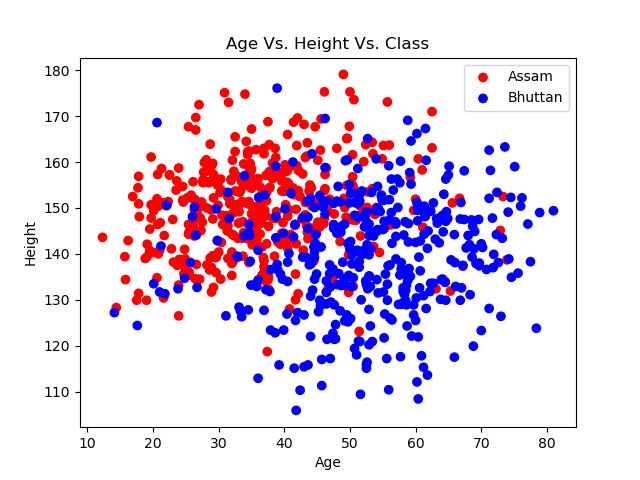
\includegraphics[width=.8\textwidth]{data_visuzlization.png} % graphic has a width of 80% of the page
    \caption{Plot Shoing Age, Height, and Snowfolk Class} % text to display with figure
    \label{fig:dataViz} % label for you to cite the figure with
\end{figure*}


% What about the [h!] at the begining of figure?
% This parameter determines where the figure will be placed, there are several options:
%
% h -- place float here
% t -- place at top of page
% b -- place at bottom of page
% p -- put on special page for floats
% ! -- do what I specify and don't optimize page layout

After you have your figure, you can refer to it like math, and tables like this: figure \ref{fig:dataViz} is cool.
Why is this cool I hear you asking? Well, if you update the graphic, you just have to place it in this folder and overwrite the old one.
You don't have to search for it in a word document.
Also if you insert a graphic above figure \ref{fig:dataViz}, you don't need to re-label anything.


\subsection{Side By Side Figures} \label{sec:sidebyside}

The command subsection is used to create a subsection. There are also commands for subsubsections.
You can also reference sections like this: section \ref{sec:sidebyside}.
We can see that section \ref{sec:sidebyside} is inside section \ref{sec:figures}.
If you want to reference a section, you have to add a label to it that is on the same line as the section command.


\begin{figure*}[h!]
    \centering
    \subfloat{{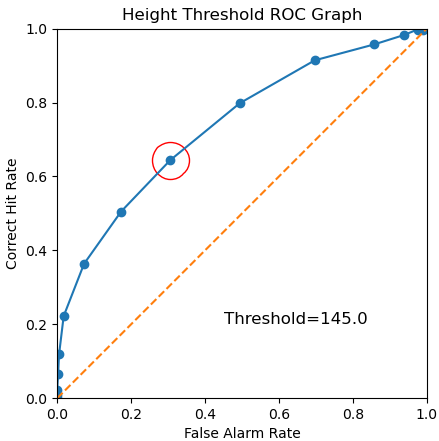
\includegraphics[width=0.45\textwidth]{height_roc_graph.png}}}%
    \qquad
    \subfloat{{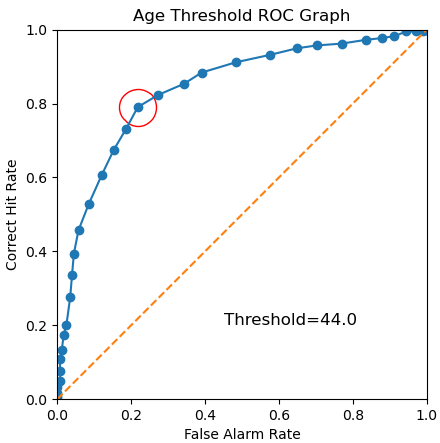
\includegraphics[width=0.45\textwidth]{age_roc_graph.png}}}%
    \caption{ROC Curves for Age and Height Classifications}%
    \label{fig:rocCurves}
\end{figure*}


Creating a side by side figure is very similar to how you would create a normal figure.
However, note that for this you need the package "subfig". Referencing this is the same:
figure \ref{fig:rocCurves}.


\subsection{Citations}

Wow, let's cite my favorite book \cite{DUMMY:1}.
It is typical to put all your bibtex citations in a file ending with the extension ".bib".
At the end of the document, you can create the bibliography using the "\\bibliography" command.
What is amazing about this is that you can then specify what type of bibilography it generates. IE: you can cite using ieee, MLA, APA, etc. This package takes care of all the formatting and ordering of your citations. Another cool thing is that, you can have loads of citations in your bib file, but, the references list will get generated using only the ones that you ended up using in your paper. 

\newpage

\bibliography{example} 
\bibliographystyle{ieeetr}

\end{document}